\chapter{Scalable User-centric cloud networking}
\ifpdf
    \graphicspath{{Chapter3/Chapter3Figs/PNG/}{Chapter3/Chapter3Figs/PDF/}{Chapter3/Chapter3Figs/}}
\else
    \graphicspath{{Chapter3/Chapter3Figs/EPS/}{Chapter3/Chapter3Figs/}}
\fi

\todo{need to update this to meet the motivation below}
In this chapter we explore application of the SDN technology in Cloud Computing.
The availability of cheap cloud computing resources, boosted the development of
a wide ecosystem of applications that aim to fulfil the needs of users to handle
efficiently and ubiquitly personal information.  We term this use case of cloud
computing as Personal Cloud (PerCl). Applications like facebook,
dropbox, google services~et.al.  abstract online user identity among devices,
associate it with information, which is disseminated based on the user policy.
Such services manage to simplify the way we use computers, but most of the times
they employ mechanisms that undermine the security and privacy of users, while
use network resources inefficiently. 

We propose an Internet-wide overlay network architecture which enables PerCl, while
addressing the aforthmentioned shortcomings. The architecture builds around an
\of controller running on end-hosts, which is enhanced with the ability to
control several off-the-self tunneling programs. The proposed architecture employs
a distributed network connectivity negotiation protocol between end-hosts, that
scales the complexity of end-system orchestration through control ditribution.

From the user perspective, the system achieves backward compatibility with
existing applications through the integration of the  architecture on the
network layer of the network stack. As a result, legacy aplications can take
advantage of the architecture by communication over a specific local
network subnet. Additionally, the proposed system exposes a simple API to
applications over the naming system, which we call {\it ``Effectful Naming''}.
Devices and user identities are represented as domain names , and an end-to-end 
path is establish through a simple name lookup. This mechanism is secured by the 
\dnssec namint service extensions. 

% The propose architecture utilizes \of-enabled bridge and a
% local controller on each device. Each controller by default forwards packets as
% normal on the local network. The forwarding logic, though,  is augmenting
% through a distributed coordination protocol which permits nodes to negotiate
% possible connection opportunities and establish ad-hoc tunnels, enabling as a
% result an Internet-wide distributed control mechanism. 
% At the core of
% our design, we  the naming service host abstraction. Each device
% acquires a global domain name, while each name resolution triggers a connection
% engine, that tries to find the best possible bidirectional channel between the
% two nodes. The naming service uses the established
% DNSSEC extension, providing a fully authenticated and secure control
% mechanism among \signpost and applications. Further, the distributed nature
% of the naming hierarchy in the Internet permits seamless control distribution.

In order to understand the feasibility and performance of the proposed
architecture we develop a strawman implementation, named {\it \signpost}.
\signpost implements the core of the control logic of the proposed architecture.
Additionally, it integrates in the architecture various network connection and
notification services.  Currently, \signpost supports SSH, OpenVPN, TOR,
NAT-punch and Privoxy connection mechanisms, while it can propagate
Multicast-DNS notifications across devices.

In the chapter we present in Section~\ref{sec:signpost-introduction} the
motivation for this work, followed then by the key observations for our design
in section~\ref{sec:signpost-design}. In
Section~\ref{sec:signpost-architecture}, we present the
architecture of our strawman implementation and it integration with existing
software. Finally, in Section~\ref{sec:signpost-evaluation}
we present a number of micro-benchmark tests for our system and conclude in
Section\ref{sec:signpost-conclusion}.

\section{Personal Clouds}\label{sec:signpost-introduction}

In the recent years, the increase in the number of networked devices per user
has created a significant information and resource management problem for
end-users. Although, each device has a specific role in the users everyday life,
the distinct roles of devices can mix, requiring resource and infromation
sharing.  For example, a smartphone is primarily a communication device. A
number of end-users though uses such devices to render audio and video content
for entertainment purposes, requiring an easy to use access mechanism to the
files of the home entertainment unit.  Such emerging requirements drive the
development of centralised device management and resource virtualization
systems. We term such systems as {\it ``Personal Clouds''}. 
A significant number of applications and protocols has been introduced
that enables seemless inter-device cooperation and provide functionalities like
remote desktop, file sharing, remote login, remote printing etc. over the
network and across devices.  Additionally the network community has also
developed a number of automation mechanisms to reduce the configuration burden.
Multicast-DNS, Universal Plug and Play and ZeroConf protocols allow a user to
browse and controll available shared services upon connection to a network.
Such mechanism are very effective when devices are collocated within the same
network and there isn't any policying in inter-device communication.
In this section we discuss the problems arising in Internet-wide Personal Clouds,
present existing approaches to the problem and discuss the goals of
Signpost abstraction.

% We term {\it ``Personal Cloud``}, the resource sharing and control abstraction
% that the user can exercise among his devices. Personal cloud is an efficient way
% for users to embrace technology and take full advantage of it. Unfortunately,
% interconnecting devices across the Internet has become increasingly difficult.

% , mainly due to the
% way that the Internet evolves.

\subsection{Challenges}

Internet is an excellent example of a dynamic system that manages to respond
effectively to the evolving user requirements.  In the early days of the system,
expand faster the user base, its design board set simplicity and openness as
fundamental design goals.  As a result, Internet protocols achieved quickly
extensive system support, while hosts could use any Internet services simply by
connecting to a network with an Internet gateway. During that period, the
Internet remained a large wide area network interconnecting research institutes
and its main use cases revolve around asynchronous communication. Through the
years, the evolution in its use cases highlighted a number of limitation on the
design of the system, a number of which related to security and performance.

In order to address these limitations in a backward compatible manner, a number
of network hacks were introduced in the Internet design. One of the most popular
hack is the deployment of middleboxes.  Middleboxes violate in a number of ways
design principles of the Internet, but they provide an effective framework to
insert in the network new functionality and address a design limitation.
NATboxes address the IPv4 address shortage, WAN optimizers improve utilization
of underprovisioned links, while firewalls secure critical networks. Middlebox
deployment has redefined to a great extend the Internet abstraction. A number of
papers have quantifies their impact.  In~\cite{Honda:2011ci} authors pinpoint
middlebox functionality as a core cause in the oscification of the transport
layer, while in~\cite{Kreibich10} authors describe the limitations that
middleboxes introduce in protocol specifications, through thorough test of some
protocol corner cases.  \todo{ describe some efforts to overcome middleboxes.}

An important impact of middlebox deployment and development is the reduced
connectivity introduced in the Internet. Home networks host a number of hidden
devices which are inaccesible from the Internet due to NATbox functionality,
while enterprise networks reduce protocol functionality through strict network
policy enforcement by network firewalls. Personal Cloud deployment across the
Internet is heavily restricted by the luck of openness.

% §develop and deploy various protocol modifications that tried to bypass these
% design flaws.  Unfortunately, such systems tend to introduce stricter
% assumptions on how the network should function, and reduce to a great extend the
% openess of the Internet.There are primarily two major classes of engineering
% modifications that reduce network connectivity: performance enhancing
% middleboxes and edge-network security policy reinforcement.  
% Performance
% enhancing middleboxes are network forwarding devices, installed in the network,
% that aggregate information from multiple layers of the TCP/IP stack and modify
% packet content or forwarding logic. 
% This restriction in openess of some parts of
% the Internet is a vital reason for the inability of the network community to
% establish Private Clouds across the Internet.  

\subsection{Approaches} 

Although Internet reachability is reduced, the system remains highly performent
and connected; it interconnect billion of users and transports terrabytes of
information everyday. This is achieved due to the predominant mode of
operation of Internet services. Hosts in the common case connect to
a small subset of the Internet hosts, that expose network services and 
provide access to popular information. 
This model, which is called {\it Client-Server model}, is a natural result of the
power law behaviour of various social and engineering mechanisms. Internet
network graph is a power law graph, due to its scalable hierarchical structure, 
while information popularity exhibits strong power law characteristics. 

Personal cloud computing is not a good match for the Client-Server model.
Personal devices most commonly are connected to networks that are optimised for
outgoing connectivity, while the Internet is not able to accommodate well-connected
services for every host. More specifically, NATed networks that can scale
connectivity on the edges of the network require manual configuration by the
administrator in order to permit hosts to expose services, while a number of
edge networks, like mobile and enterprise networks, restrict publicly accessible
services on connected hosts. In order to overcome these restrictions a number of
approach has been proposed by the research community as well as the industry. We
group these solutions in the following two categories:

\paragraph*{Decentralised Personal Cloud}: 

Numerous frameworks have been proposed over the years that use publicly
available services and provide bidirectional connectivity between devices. We
are considering in this category tunneling software, like OpenVpn and SSH, and
NAT and firewall punching mechanism, like STUN. Although such mechanisms are
effective in a number of scenarios, a number of assumption and configuration
requirements dim them inappropriate for inexperienced users. As we have already
discussed in Section~\ref{s:home_social} average Internet user is willing to
configure its network service n as long as the configuration tasks are short
and simple. Establishing connectivity through user-managed
mechanisms is not straightforward. Functionality contains assumptions on the
connectivity of the environment and users have to resolve to ``try and error''
approaches to check which mechanism can be effective in a specific environment,
while prior configurations in required in a number of different subsystems of the 
network. 

As an example, we describe the steps required by a user to establish
connectivity using the SSH service. Before the user is able to connect to a
computer using SSH, he has to configure the service on his local machine, the
security credentials on the server and any firewall and NATbox deployed in the
network. Upon connection, the user has to run the SSH client, choose the ports
he is interested to forward and configure the connecting software to use them.
This connectivity is subject to the ability of the user in the remote network to
use the SSH protocol on the preconfigure port.  In case this is not possible,
the user has to resolve to a different service.

\paragraph*{cloud-assisted Personal Cloud}:

% According to wikipedia~\cite{wiki-cloud}, the definition of {\it ``Cloud''} is:
% \begin{quote}
%   Cloud computing is the use of computing resources (hardware and software) that
%   are delivered as a service over a network (typically the Internet). 
% \end{quote}
% The {\it``Coud''} has been a buz world that receive increased attention within
% the recent years.  The concept is not novel for the computer science community,
% and can be placed under the generic engineering technique of abstraction and
% virtualisation. Its popularity though can be mapped to theeffectiveness of the
% abstraction as well as the increased interest in distributed large data
% processing infrustructure.  Interestingly, the initial idea for cloud computing
% aimed to create a small scale economical market that would take advantage of
% iddle data center resources, but the model became so successful that companies
% create new data center infrustructure solely to support this service. 

% Our work in this chapter aims to revisit the design of cloud applications that
% target end-users and provides them the ability to store and share
% information. Such application usually consist of 2 layers of abstraction, which
% oftenly are not controlled by the same entity. In the lower layer of the system
% we find the infrastructure abstraction layer, which is usally termed as
% {\it Infrustructure as a Service}. This service is controlled by the
% entity that controls the data center and ensures and enforce the required resource
% allocations over the available hardware. Usually, this relies on the management
% of a large number of commodity servers running an OS virtualisation framework,
% like Xen, and configure the network in order to match the resource
% virtualization mechanisms. At the upper layer of the system, we find the service
% abstraction layer, which is also called as the {\it Software as a Service} or
% {\it Platform as a Service}. This layer provides the resulting abstraction to
% the user, and it main focus is to translate the required functionality
% by the user into a number of distributed computations that can be distributed
% over the abstraction of machines that the lower layer provides. In most of the
% cases, the end-user of a cloud application is usually exposed  directly only to
% the upper layer of the afortmentioned abstractions. 

% Cloud computing mechanisms have managed to provide a sufficient platform that
% can accomodate the processign requirements for a large number of applications,
% while it also provides ways to scale systems very fast in order to support
% emerging applications. The main architectural approach that has been used in
% order to achieve is to direct users to a centrally controlled system. User copy
% their data to the public cloud infrustructure and interact with the public API
% of the service. The service provider can post analyse the user data in order to
% create the intermediate data required in order to provide timely responsiveness
% for its service.

An alternative approach which has been highly succesful in the recent years uses
third party services to establish inter-device connectivity.  In this class we
consider cloud applications like google service suite and
Dropbox. Such approaches have managed to provide a simple and intuitive
abstraction to users, while taking advantage the development in cloud
infrastructures, they provide high performance. Although this approach can be
characterised as successful in providing connectivity, some properties remain
ambivalent and demotivate user engagement. 

\begin{itemize}
  \item{\it authentication}: cloud applications provide an effective
       framework to control information dissemination between devices and
       users.  Users can define an access policy based on online identities 
       and the service will ensure secure delivery of information.  This
       mechanism though introduces privacy concerns, as the authentication
       mechanisms can be employed in online user identification and monitoring. 
       In~\cite{Krishnamurthy2009} authors reports cases of online OSN that leak
       information to ad services in order to detect and characterize
       individuals, while Facebook has openly verified the existence of such
       services~\footnote{\url{http://en.wikipedia.org/wiki/Facebook_Beacon}}. 

% \paragraph*{authentication}: A number of cloud applications provide an effective framework
% to control information dissemination between devices as well as users. 
% Users are required solely to verify that an online identity is a valid destination for
% an information quantum. The platform will ensure that the information will be
% accessible only to users that have the valid credentials for that account in any
% time, easing the information access control from end-users. This mechanism has
% been further used by other application to offload their authentication mechanism
% to a third party cloud service. This mechanism though has been reported to be
% abused by some service providers. In~\cite{Krishnamurthy2009} authors reports
% cases of online OSN that leak information to ad services which allows them to
% detect and characterize individuals. This was recognized by facebook as a paid
% service provide to ad services and removed after wide privcacy concerns by
% users~\footnote{\url{http://en.wikipedia.org/wiki/Facebook_Beacon}}. The wide
% adoption of such authentication mechanisms raises concerns for the control of
% the privacy of users.  
% On the other hand though, it has been reported that some cloud
% applications have engaged in leaking information on users to third party
% application. A study in~\todo{add reference} reports that the social network
% facebook leaks identity hints to advrtising platforms in order to enhance their
% ability to characterise users, a functionality which is privacy envasing for
% some users. 

\item {\it performance}: Cloud services manage to deliver user acceptable
      performance to million of users across the world. Google claims that any
      user is in range of a few thousand of mile of at least a single google
      datacenter. Although this approach provides user satisfying service
      performance, it is wasteful in processing resources; Cloud services under
      utilize rich edge resources. Two devices that are behind the same subnet
      will suffer from increased RTT values when communicating using a cloud service,
      while public cloud storage cost and performance is orders of magnitude
      worser than local network file services. In~\cite{Wittie2010}, authors
      report a significant impact on the 95th quantile network
      performance of cloud services, due to latency and packet losses incurred
      by the Internet. 
% \paragraph*{performance}: A number of cloud services manage to deliver user
% acceptable performance to million of users across the world. This is achieved to
% a great extend by careful design of data processing pipelines, that paralelize
% processing logic and preemptively calculate results for future user requests.
% Additionally, large service providers develop global distribution networks with
% multiple entry points close to the user.  Google claims that any user is in
% range of a few thousand of mile of at least a signle google datacenter. Although
% this approach provides a user satisfying service performance, it is wasteful in
% processing resources; Cloud services under utilize rich edge resources. Two
% devices that are behind the same subnet and communicate using a cloud service 
% have to communicate through the datacenter infrustructure of the provider, 
% increasing significantly latency. Additionally, public cloud storage cost is two
% orders of magnitude more expensive that the cost to maintain data on your local
% disk. 
% Finally, a number of measurement studies have highlighted a significant impact
% on the 95th quantile performance of cloud services, due to latency and packet
% losses incurred by the Internet~\cite{Wittie2010}. 

\item {\it cost}: Free cloud services have an interesting 3-party economical
      model that uses advertisement as a mechanism to cover the 
      infrastructural costs. The providers though, due to the free nature of the service,
      provide very weak user SLA's. If a part of the service is compromised and
      information is leaked, the service provider bears no obligation
      towards affected users. Such costs are not directly observed by the
      end-user, but they may impact significantly his social and work experience. 
      \todo{report Dropbox problem}
% \paragraph*{cost}: Free cloud services have an interesting 3-party economical
% model that uses advertisment as a mechanism to circulate capital and sustain the
% cost of the infrustructure. As a result, users are able to enjoy high quality
% services with minimum costs. The SLA's though, because of the free nature of the
% service are not wiling to provide any SLA's to users. If a part of the service
% is compromised and some information is leaked, then the service provider bears
% no obligation towards affected users. Such costs are not directly observed by
% the end-user, but they may impact significantly his everyday life. 

\item {\it Availability}: Cloud services run on well connected infrastructures
      with a large number of network engineers ensuring security and
      performance.  Any device with Internet connectivity is able to connect to
      the cloud service using default settings. Further, cloud services function
      as an always accessible cache between devices and users.  Devices though
      are unable to interconnect and access shared information, if Internet
      connectivity is unavailable, even if they are able to interconnect on the
      network layer.  Two users behind the same firewall will never be able to
      exchange a file over dropbox, if the network policy forbids any connection
      with the servers of the service. 
% \paragraph*{Availability}: As we have already discussed in the Introduction of
% this thesis, Internet has reduced significantly the bidirectional connection
% property of Internet hosts. The deployment of performance-enhancing middleboxes
% makes highly impossible for a device to expose an Internet-wide service.
% Additionally, the large number of malicious nodes that try to exploit security
% vulnerabilities, is counter intuitive for users. Cloud service providers address
% this problem in a highly effective manner. Their network default policy is
% permit, while a handful of network engineers are constantly monitoring the
% security of the datacenter and ensure high availability of the system and data
% integrity.  As a result, any device with Internet connectivity is able to
% connect to the service, without any special configuration of the OS or the
% Network policy. Cloud services function as a proxy between devices and users,
% that provides them connectivity in most cases. Although, the centralised
% design of such services makes it impossible for devices to interconnect when
% there isn't any Internet connectivity. Two users behind the same firewall will
% never be able to exchange a file over dropbox, if the network policy forbids
% any connection with the servers of the service. 
\item {\emph Generality}: 

\end{itemize}

\todo{A large set of protocol to coordinate distributely home networks. }

\subsection{Reconnecting the Internet}\label{sec:signpost-design}

In order to model the problem of Personal Cloud network connectivity, we propose
a system that fuses existing approaches. Our system design goals are twofold.
Firstly, we develop a user friendly framework that automates connectiion
configuration. In order to achieve this, we model the way various existing 
decentralised mechanisms establish connectivity and encode their configuration 
and assumptions testing in a generic
automation framework. Further, the system reuses existing network abstractions which are
intuitive to Internet users. The connection establishment mechanism exports
connectivity through the network layer abstraction, allowing existing
applications to take advantage of the system. Further, we reuse the naming
abstraction of the DNS service; each device has a user-defined domain name under
the signpo.st domain.  Secondly, the system exposes a user-controlled security
mechanism, which can provide different security properties on connections
between devices. As a result, the user is able to fully control the
dissemination of his information, without relying his policy enforcing mechanism
on the service provider or leaking any privacy-sensitive information to a third
party entity. 

\begin{figure}[ht]
  \begin{center}
	\includegraphics[width=0.6\textwidth]{signpost-illustration}
  \end{center}
  \caption{A simple example of the Signpost abstraction when the user Alice
    interconnects a smarthphone with the home computer over the Internet.}
  \label{fig:signpost-user-abstraction}
\end{figure}

A schematic of the abstraction that our system provides to end-users is depicted
in Figure~\ref{fig:signpost-user-abstraction}. In this scenario user Alice, who
is at work and uses her smartphone, wishes to access some files from her laptop
which is behind the NATed home router. In order to express her interest to
connect to her laptop, the user needs solely to perform a name lookup for the
domain name home.alice.signpost.io. The name lookup will propagate through the
DNS infrastructure to the cloud presence of her signpost system. The Signpost
server will trigger the two devices to try any possible network tactic and try
to establish an end-to-end path between the two devices. Once the server has
ensured that a first channel has been establish, it will reply to the initial
DNS query with a local IP address which will be routed by the local Network
stack to the tunnel between the two devices. In parallel, the server will
continue recursively to test different tactics in case a better connection can
be established. 

% Our work builds on the observations on the shortcoming of current approaches to
% interconnect devices, and tries to bridge the two domains, providing the
% appropriate control mechanisms to end-users. On one hand, we want to
% model a generic framework that will allow end-host to automatically test the
% network environment, discover the optimum mechanism to interconnect two
% devices and distributely negotiate the connection parameters with other devices,
% without any user interaction. On the other hand, we want to provide to the users
% a mechanism that will allow them to control to a great extend the security and
% privacy of their information. 

\section{Signpost Architecture}\label{sec:signpost-architecture}

\begin{figure}[ht]
  \begin{center}
	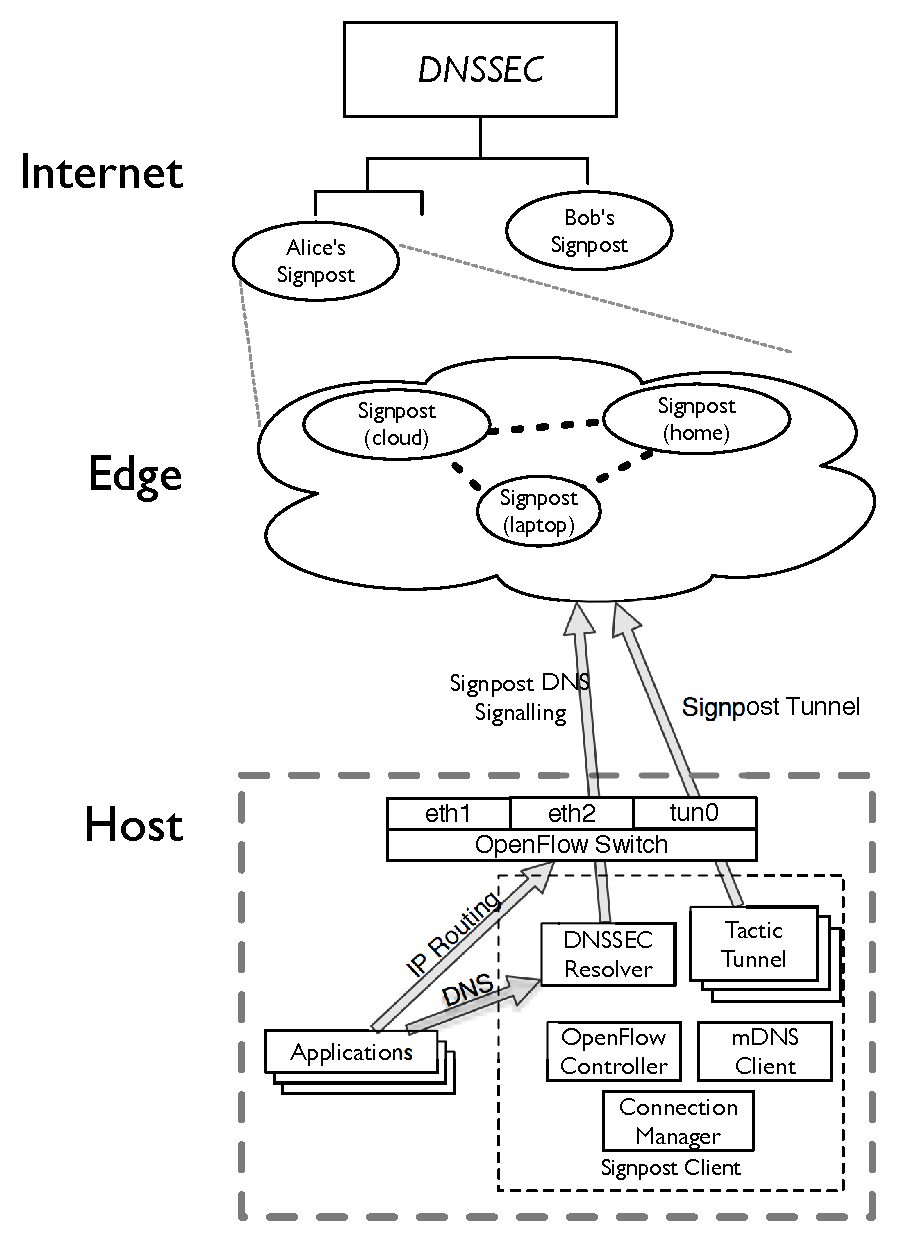
\includegraphics[width=0.6\textwidth]{signpost-arch}
  \end{center}
  \caption{Signpost architecture }
  \label{fig:signpost-arch}
\end{figure}

In order to implement the proposed architecture we develop a strawman
implementation of the platform, named Signpost. Signpost touched three main
points: Naming service, connection engine, tactic and forwarding. We further
describe changes for each point in the system. 

\subsection{Network Tactic}

\subsection{Connection Manager}

\subsection{}<++>

\section{Security}

\todo{\dnssec description}
\todo{Effectful naming}
\todo{How \signpost looks like to the outside}

\todo{Connection Engine}

\todo{Tactic life cycle}

We propose a novel overlay network architecture that enables PCC while
minimizing the interaction with the cloud infrustructure. 
The propose architecture utilizes \of-enabled bridge and a
local controller on each device. Each controller by default forwards packets as
normal on the local network. The forwarding logic, though,  is augmenting
through a distributed coordination protocol which permits nodes to negotiate
possible connection opportunities and establish ad-hoc tunnels, enabling as a
result an Internet-wide distributed control mechanism. At the core of
our design, we tranform the naming service host abstraction. Each device
acquires a global domain name, while each name resolution triggers a connection
engine, that tries to find the best possible bidirectional channel between the
two nodes. The naming service uses the established
DNSSEC extension, providing a fully authenticated and secure control
mechanism among \signpost and applications. Further, the distributed nature
of the naming hierarchy in the Internet permits seamless control distribution.

In order to understand the impact of the proposed architecture we develop a
strawman implementation, named {\it Signpost}. Signpost implements the core of
the control logic of the proposed architecture. Additionally, it integrades a
number of network tactics of established tunneling and notification mechanisms.
Currently \signpost provides integration of the main architecture with SSH, OpenVPN,
TOR, Privoxy, Multicast-DNS and Nat punching. 


\section{Evaluation}\label{sec:signpost-evaluation}

\section{Conclusions}\label{sec:signpost-conclusion}
%\section{Second Section}
%\markboth{\MakeUppercase{\thechapter. My Second Chapter }}
%and here I write more ...
%
%\subsection{first subsection in the Second Section}
%... and some more ...
%
%\subsection{second subsection in the Second Section}
%... and some more ...
%
%\subsection{third subsection in the Second Section}
%... and some more ...

% ------------------------------------------------------------------------

%%% Local Variables: 
%%% mode: latex
%%% TeX-master: "../thesis"
%%% End: 
